\part{Swoole}



\chapter{Introduction}


Swoole是一种基于PHP核心开发的高性能网络通信框架\footnote{Swoole本质是PHP的一种异步并行扩展,因此要应用Swoole,首先需要有PHP环境。},提供了PHP语言的异步多线程服务器,异步TCP/UDP网络客户端,异步MySQL,异步Redis、数据库连接池,AsyncTask,消息队列,毫秒定时器,异步文件读写,异步DNS查询。

Swoole内置了Http/WebSocket服务器/客户端、Http2.0服务器。

\begin{compactitem}
\item swoole\_server,高并发高性能功能强大的异步并行TCP/UDP Server。
\item swoole\_client,支持同步/异步/并发的socket客户端实现\footnote{Swoole内置了Socket客户端的实现,但是采用的是同步+并行方式来执行。PHP本身虽然也提供了socket的功能,但是某些函数存在bug,而且比较复杂,因此使用Swoole内置的客户端类更加安全和简化。}。
\item swoole\_event,基于epoll/kqueue的全自动IO事件发生器。
\item swoole\_task,基于进程池实现的异步任务处理器。
\end{compactitem}

其中,swoole\_event比libevent更简单,仅需add/set/del几个操作即可,这样使用者就可以将原有PHP代码中的streams/fsockopen/sockets代码加入到swoole实现异步化,而且利用swoole\_event还可以实现真正的PHP异步MySQL。

用户可以使用swoole\_task实现PHP的数据库连接池,慢操作异步化\footnote{Swoole使用了传统Linux下半同步半异步多Worker的实现方式,业务代码可以按照更简单的同步方式编写,只有慢操作才考虑使用异步。},可以说Swoole开始将多线程、异步、阻塞引入PHP应用开发。

实际上,Swoole底层内置了异步非阻塞、多线程的网络IO服务器,这样仅需处理事件回调\footnote{如果在使用Node.js等进行开发时的代码太复杂,就会产生嵌套多层回调,使代码丧失可读性,程序流程变得很乱。}即可,无需关心底层。

与Nginx/Tornado/Node.js等全异步的框架不同,Swoole既支持全异步\footnote{Node.js支持全异步回调,而且内置了异步高性能的Socket Server/Client实现,在此基础上提供了内置的Web服务器。},也支持同步(或者半异步半同步)。

除了异步IO的支持之外,Swoole为PHP多进程的模式设计了多个并发数据结构和IPC通信机制,可以大大简化多进程并发编程的工作。其中包括了并发原子计数器,并发HashTable,Channel,Lock,进程间通信IPC等丰富的功能特性。


\section{Overview}

最初,PHP在每个请求进来后都需要重新初始化资源,并且在请求执行完毕后全部丢弃,不过在CLI模式下可以不释放资源。



\section{FastCGI}



\section{Multithread}

同步和多线程的关系如下:

\begin{compactenum}
\item 没有多线程环境就不需要同步。
\item 即使有多线程环境也不一定需要同步。 
\end{compactenum}




\subsection{Block}


一旦一个线程处于一个标记为synchronized的方法中,那么在这个线程从该方法中返回之前,其他所有要调用类中任何标记为synchronized方法的线程都会被阻塞。  




每个对象都有一个单一的锁,这个锁本身就是对象的一部分。

当在对象上调用其任意synchronized方法的时候,此对象都被加锁,这时该对象上的其他synchronized方法只有等到前一个方法调用完毕并释放了锁之后才能被调用。

原子操作不需要进行同步(对除double和long以外的其他基本类型的进行读取或赋值的操作也是原子操作),然而只要给long或double加上volatile,操作就是原子操作了。

只能在同步控制方法或同步块中调用wait()、notify()和notifyAll()。如果在非同步的方法里调用这些方法,在运行时会抛出java.lang.IllegalMonitorStateException异常。 

\begin{compactitem}
\item  在调用wait的时候,线程自动释放其占有的对象锁,同时不会去申请对象锁。
\item 当线程被唤醒的时候,它才再次获得了去获得对象锁的权利。其中:

\begin{compactenum}
\item notify仅唤醒一个线程并允许它去获得锁;
\item notifyAll是唤醒所有等待这个对象的线程并允许它们去获得对象锁。
\end{compactenum}

\end{compactitem}





\subsection{Dispatch}



OOP 的实现相对来说比较复杂,如果低层实现不好,用户的感受只能是难以使用,因此为了保证效率同时避免不必要的运行判定,有以下两个问题一定解决:

\begin{compactitem}
\item 调度(Dispatch):相对于静态判定,当调度和重新调度时,在程序执行时动态决定所要调用的子程序。
\item 多继承(Multiple Inheritance):从两个或更多的父类型中继承成员及操作。
\end{compactitem}



\section{MultiProcess}



\section{Synchronization}




\section{Asynchronization}






\chapter{Installation}

swoole是标准的PHP扩展,而且不依赖PHP的stream、sockets、pcntl、posix、sysvmsg等扩展,因此只需下载Swoole源码包并解压至本地任意目录(保证读写权限)来进行编译安装,PHP则只需安装最基本的扩展即可。

按照PHP标准扩展构建的构建流程,首先使用\texttt{phpize}\footnote{phpize命令需要autoconf工具,需要预先安装。}来生成PHP编译配置,然后执行\texttt{./configure}来做编译配置检测,\texttt{make}进行编译,\texttt{make install}进行安装。

除了手工下载编译外,还可以通过PHP官方提供的pecl命令来在线安装swoole:

\begin{lstlisting}[language=bash]
# pecl install swoole
# pecl upgrade swoole
$ php --ri swoole
\end{lstlisting}



\section{Linux}


在安装PHP前,需要安装编译环境和PHP的相关依赖\footnote{swoole编译为libswoole.so作为C/C++库时需要使用cmake。}。



\begin{lstlisting}[language=bash]
$ sudo apt-get install \
	build-essential  \
	gcc \
	g++ \
	autoconf \
	libiconv-hook-dev \
	libmcrypt-dev \
	libxml2-dev \
	libmysqlclient-dev \
	libcurl4-openssl-dev \
	libjpeg8-dev \
	libpng12-dev \
	libfreetype6-dev
\end{lstlisting}

如果在CentOS/RHEL环境下编译安装PHP,则需要预先执行:


\begin{compactenum}
\item 编译环境


\begin{lstlisting}[language=bash]
$ sudo yum -y install \
	gcc \
	gcc-c++ \
	autoconf \
	libjpeg \
	libjpeg-devel \
	libpng \
	libpng-devel \
	freetype \
	freetype-devel \
	libxml2 \
	libxml2-devel \
	zlib \
	zlib-devel \
	glibc \
	glibc-devel \
	glib2 \
	glib2-devel \
	bzip2 \
	bzip2-devel \
	ncurses \
	ncurses-devel \
	curl \
	curl-devel \
	e2fsprogs \
	e2fsprogs-devel \
	krb5 \
	krb5-devel \
	libidn \
	libidn-devel \
	openssl \
	openssl-devel \
	openldap \
	openldap-devel \
	nss_ldap \
	openldap-clients \
	openldap-servers \
	gd \
	gd2 \
	gd-devel \
	gd2-devel \
	perl-CPAN \
	pcre-devel
\end{lstlisting}

\item 编译PHP


\begin{lstlisting}[language=bash]
$ cd /usr/local/php-src
$ ./configure \
	--prefix=/usr/local/php \
	--with-config-file-path=/etc/php \
	--enable-fpm \
	--enable-pcntl \
	--enable-mysqlnd \
	--enable-opcache \
	--enable-sockets \
	--enable-sysvmsg \
	--enable-sysvsem \
	--enable-sysvshm \
	--enable-shmop \
	--enable-zip \
	--enable-ftp \
	--enable-soap \
	--enable-xml \
	--enable-mbstring \
	--disable-rpath \
	--disable-debug \
	--disable-fileinfo \
	--with-mysql=mysqlnd \
	--with-mysqli=mysqlnd \
	--with-pdo-mysql=mysqlnd \
	--with-pcre-regex \
	--with-iconv \
	--with-zlib \
	--with-mcrypt \
	--with-gd \
	--with-openssl \
	--with-mhash \
	--with-xmlrpc \
	--with-curl \
	--with-imap-ssl
$ sudo make
$ sudo make install
$ sudo cp php.ini-development /etc/php/
$ cat >> ~/.bashrc
export PATH=/usr/local/php/bin:$PATH
export PATH=/usr/local/php/sbin:$PATH

$ source ~/.bashrc
$ php --version
PHP 5.6.12 (cli) (built: Aug 31 2015 11:09:49) 
Copyright (c) 1997-2015 The PHP Group
Zend Engine v2.6.0, Copyright (c) 1998-2015 Zend Technologies
\end{lstlisting}

\item 编译swoole

\begin{lstlisting}[language=bash]
$ cd /usr/local/src/
$ sudo tar zxvf swoole-1.7.19-stable.tar.gz
$ cd swoole-src-swoole-1.7.19-stable
$ sudo phpize
$ sudo ./configure \
	--enable-openssl \
	--enable-swoole-debug \
	--enable-ringbuffer \
	--with-php-config=/usr/local/bin/php-config \
	--enable-async-mysql=/usr/local/mysql \
	--with-swoole \
	--enable-swoole \
	--with-gnu-ld \
	--with-pic
$ sudo make
$ sudo make install
$ sudo echo "extension=swoole.so" >>  /usr/local/lib/php.ini
$ php -m
[PHP Modules]
Core
ctype
date
dom
ereg
filter
hash
iconv
json
libxml
mysql
mysqlnd
pcre
PDO
pdo_sqlite
Phar
posix
propro
raphf
Reflection
session
SimpleXML
SPL
sqlite3
standard
swoole
tokenizer
xml
xmlreader
xmlwriter

[Zend Modules]
\end{lstlisting}

\item 查看swoole信息

\begin{lstlisting}[language=bash]
# php --ri swoole
swoole
swoole support => enabled
Version => 1.7.19
Author => tianfeng.han[email: mikan.tenny@gmail.com]
epoll => enabled
eventfd => enabled
timerfd => enabled
signalfd => enabled
cpu affinity => enabled
spinlock => enabled
rwlock => enabled
sockets => enabled
openssl => enabled
ringbuffer => enabled
Linux Native AIO => enabled
Gcc AIO => enabled
pcre => enabled
zlib => enabled
mutex_timedlock => enabled
pthread_barrier => enabled

Directive => Local Value => Master Value
swoole.aio_thread_num => 2 => 2
swoole.display_errors => On => On
swoole.message_queue_key => 0 => 0
swoole.unixsock_buffer_size => 8388608 => 8388608
\end{lstlisting}
\end{compactenum}



通过\texttt{php -m}\footnote{首先查看加载的php.ini路径并确认加载了正确的php.ini,其次可以使用绝对路径指定swoole的位置,最后在php.ini中打开错误显示来检查是否存在启动时错误。}或\texttt{phpinfo()}来查看是否成功加载了swoole,如果没有可能是php.ini的路径不对,可以使用\texttt{php -i |grep php.ini}来定位到php.ini的绝对路径。

\subsection{Error}


修改php.ini,打开错误显示,查看是否存在启动时错误。

\begin{lstlisting}[language=bash]
display_errors => Off => Off
display_startup_errors => Off => Off
html_errors => Off => Off
ignore_repeated_errors => Off => Off
log_errors => On => On
log_errors_max_len => 1024 => 1024
track_errors => Off => Off
xmlrpc_errors => Off => Off
swoole.display_errors => On => On
\end{lstlisting}

默认情况下,可以在php.ini修改错误报告的设置,例如:

\begin{lstlisting}[language=bash]
;;;;;;;;;;;;;;;;;;;;;;;;;;;;;;
; Error handling and logging ;
;;;;;;;;;;;;;;;;;;;;;;;;;;;;;;

; This directive informs PHP of which errors, warnings and notices you would like
; it to take action for. The recommended way of setting values for this
; directive is through the use of the error level constants and bitwise
; operators. The error level constants are below here for convenience as well as
; some common settings and their meanings.
; By default, PHP is set to take action on all errors, notices and warnings EXCEPT
; those related to E_NOTICE and E_STRICT, which together cover best practices and
; recommended coding standards in PHP. For performance reasons, this is the
; recommend error reporting setting. Your production server shouldn't be wasting
; resources complaining about best practices and coding standards. That's what
; development servers and development settings are for.
; Note: The php.ini-development file has this setting as E_ALL. This
; means it pretty much reports everything which is exactly what you want during
; development and early testing.
;
; Error Level Constants:
; E_ALL             - All errors and warnings (includes E_STRICT as of PHP 5.4.0)
; E_ERROR           - fatal run-time errors
; E_RECOVERABLE_ERROR  - almost fatal run-time errors
; E_WARNING         - run-time warnings (non-fatal errors)
; E_PARSE           - compile-time parse errors
; E_NOTICE          - run-time notices (these are warnings which often result
;                     from a bug in your code, but it's possible that it was
;                     intentional (e.g., using an uninitialized variable and
;                     relying on the fact it is automatically initialized to an
;                     empty string)
; E_STRICT          - run-time notices, enable to have PHP suggest changes
;                     to your code which will ensure the best interoperability
;                     and forward compatibility of your code
; E_CORE_ERROR      - fatal errors that occur during PHP's initial startup
; E_CORE_WARNING    - warnings (non-fatal errors) that occur during PHP's
;                     initial startup
; E_COMPILE_ERROR   - fatal compile-time errors
; E_COMPILE_WARNING - compile-time warnings (non-fatal errors)
; E_USER_ERROR      - user-generated error message
; E_USER_WARNING    - user-generated warning message
; E_USER_NOTICE     - user-generated notice message
; E_DEPRECATED      - warn about code that will not work in future versions
;                     of PHP
; E_USER_DEPRECATED - user-generated deprecation warnings
;
; Common Values:
;   E_ALL (Show all errors, warnings and notices including coding standards.)
;   E_ALL & ~E_NOTICE  (Show all errors, except for notices)
;   E_ALL & ~E_NOTICE & ~E_STRICT  (Show all errors, except for notices and coding standards warnings.)
;   E_COMPILE_ERROR|E_RECOVERABLE_ERROR|E_ERROR|E_CORE_ERROR  (Show only errors)
; Default Value: E_ALL & ~E_NOTICE & ~E_STRICT & ~E_DEPRECATED
; Development Value: E_ALL
; Production Value: E_ALL & ~E_DEPRECATED & ~E_STRICT
; http://php.net/error-reporting
error_reporting = E_ALL & ~E_DEPRECATED & ~E_STRICT

; This directive controls whether or not and where PHP will output errors,
; notices and warnings too. Error output is very useful during development, but
; it could be very dangerous in production environments. Depending on the code
; which is triggering the error, sensitive information could potentially leak
; out of your application such as database usernames and passwords or worse.
; For production environments, we recommend logging errors rather than
; sending them to STDOUT.
; Possible Values:
;   Off = Do not display any errors
;   stderr = Display errors to STDERR (affects only CGI/CLI binaries!)
;   On or stdout = Display errors to STDOUT
; Default Value: On
; Development Value: On
; Production Value: Off
; http://php.net/display-errors
display_errors = Off

; The display of errors which occur during PHP's startup sequence are handled
; separately from display_errors. PHP's default behavior is to suppress those
; errors from clients. Turning the display of startup errors on can be useful in
; debugging configuration problems. We strongly recommend you
; set this to 'off' for production servers.
; Default Value: Off
; Development Value: On
; Production Value: Off
; http://php.net/display-startup-errors
display_startup_errors = Off

; Besides displaying errors, PHP can also log errors to locations such as a
; server-specific log, STDERR, or a location specified by the error_log
; directive found below. While errors should not be displayed on productions
; servers they should still be monitored and logging is a great way to do that.
; Default Value: Off
; Development Value: On
; Production Value: On
; http://php.net/log-errors
log_errors = On

; Set maximum length of log_errors. In error_log information about the source is
; added. The default is 1024 and 0 allows to not apply any maximum length at all.
; http://php.net/log-errors-max-len
log_errors_max_len = 1024
; Do not log repeated messages. Repeated errors must occur in same file on same
; line unless ignore_repeated_source is set true.
; http://php.net/ignore-repeated-errors
ignore_repeated_errors = Off

; Ignore source of message when ignoring repeated messages. When this setting
; is On you will not log errors with repeated messages from different files or
; source lines.
; http://php.net/ignore-repeated-source
ignore_repeated_source = Off

; If this parameter is set to Off, then memory leaks will not be shown (on
; stdout or in the log). This has only effect in a debug compile, and if
; error reporting includes E_WARNING in the allowed list
; http://php.net/report-memleaks
report_memleaks = On

; This setting is on by default.
;report_zend_debug = 0

; Store the last error/warning message in $php_errormsg (boolean). Setting this value
; to On can assist in debugging and is appropriate for development servers. It should
; however be disabled on production servers.
; Default Value: Off
; Development Value: On
; Production Value: Off
; http://php.net/track-errors
track_errors = Off

; Turn off normal error reporting and emit XML-RPC error XML
; http://php.net/xmlrpc-errors
;xmlrpc_errors = 0

; An XML-RPC faultCode
;xmlrpc_error_number = 0

; When PHP displays or logs an error, it has the capability of formatting the
; error message as HTML for easier reading. This directive controls whether
; the error message is formatted as HTML or not.
; Note: This directive is hardcoded to Off for the CLI SAPI
; Default Value: On
; Development Value: On
; Production value: On
; http://php.net/html-errors
html_errors = On
; If html_errors is set to On *and* docref_root is not empty, then PHP
; produces clickable error messages that direct to a page describing the error
; or function causing the error in detail.
; You can download a copy of the PHP manual from http://php.net/docs
; and change docref_root to the base URL of your local copy including the
; leading '/'. You must also specify the file extension being used including
; the dot. PHP's default behavior is to leave these settings empty, in which
; case no links to documentation are generated.
; Note: Never use this feature for production boxes.
; http://php.net/docref-root
; Examples
;docref_root = "/phpmanual/"

; http://php.net/docref-ext
;docref_ext = .html

; String to output before an error message. PHP's default behavior is to leave
; this setting blank.
; http://php.net/error-prepend-string
; Example:
;error_prepend_string = "<span style='color: #ff0000'>"

; String to output after an error message. PHP's default behavior is to leave
; this setting blank.
; http://php.net/error-append-string
; Example:
;error_append_string = "</span>"

; Log errors to specified file. PHP's default behavior is to leave this value
; empty.
; http://php.net/error-log
; Example:
;error_log = php_errors.log
; Log errors to syslog (Event Log on Windows).
;error_log = syslog

;windows.show_crt_warning
; Default value: 0
; Development value: 0
; Production value: 0
\end{lstlisting}


\subsection{Debug}


如果编译时使用了\texttt{--enable-swoole-debug},在初始化服务的时候可以set 是否debug,这样就可以在开发阶段输出调试数据。



\subsection{Xdebug}

PHP的xdebug(或Zend的zend\_xdebug\footnote{如果出现\texttt{error: too many arguments to function 'zend\_exception\_error'}错误,则说明PHP版本号低于5.3.10。})扩展都可能会swoole崩溃,运行swoole程序时务必去掉xdebug扩展。

另外,如果make或make install无法执行或编译错误,原因可能是php版本和编译时使用的phpize和php-config不对应,需要使用绝对路径来进行编译。使用绝对路径执行PHP。

\begin{lstlisting}[language=bash]
NOTICE: PHP message: PHP Warning: PHP Startup: swoole: Unable to initialize module
Module compiled with module API=20090626
PHP compiled with module API=20121212
These options need to match
in Unknown on line 0
$ sudo /usr/local/php-5.4.17/bin/phpize \
	./configure \
	--with-php-config=/usr/local/php-5.4.17/bin/php-config \
	/usr/local/php-5.4.17/bin/php server.php
\end{lstlisting}


\subsection{MySQL}


如果出现“缺少mysql头文件”错误,说明\texttt{--enable-async-mysql}需要指定路径,需要在编译前执行:

\begin{lstlisting}[language=bash]
# ./configure 
	--with-php-config=/usr/local/bin/php-config \
	--enable-sockets \
	--enable-async-mysql=/usr/local/mysql
\end{lstlisting}

如果出现“缺少mysqli头文件”错误,说明没有找到mysqlclient的头文件,需要安装mysqlclient-dev。

\begin{lstlisting}[language=bash]
php_mysqli_structs.h:64:23: fatal error: my_global.h: No such file or directory
\end{lstlisting}


建议自行编译PHP,不要使用Linux包管理系统自带的php版本,或者可以更全面的配置MySQL相关信息,如下面示例中所示:


\begin{lstlisting}[language=bash]
# LDFLAGS="-L/usr/local/mysql/lib" \
	CPPFLAGS="-I/usr/local/mysql/include" \
	./configure \
	--with-php-config=/usr/local/php/bin/php-config \
	--enable-async-mysql=/usr/local/mysql/include \
	--enable-swoole \
	--with-swoole \
	--enable-openssl \
	--enable-ringbuffer \
	--enable-sockets=/usr/local/php/ext/sockets \
	--enable-swoole-debug
\end{lstlisting}

\subsection{PCRE}

如果出现“缺少pcre.h头文件”错误,原因是缺少pcre,需要安装libpcre。


\begin{lstlisting}[language=bash]
fatal error: pcre.h: No such file or directory
\end{lstlisting}

\section{ARM}


swoole也可以运行在ARM平台,在编译Swoole时手工修改Makefile去掉\texttt{-O2}编译参数。

\section{Windows}


从swoole-1.7.7开始,swoole增加了对cygwin环境的支持,在Windows环境下可以直接使用cygwin + php 来运行swoole程序。

\begin{compactitem}
\item 安装cygwin,并安装gcc、make、autoconf、php\footnote{cygwin模式下需要对PHP进行简化,去掉不使用的扩展,避免进程占用内存过大,导致Fork操作失败。}。
\item 下载swoole源码,在cygwin-shell中进行\texttt{phpize/configure/make/make install}。
\item 修改php.ini,加入swoole.so。
\end{compactitem}




\chapter{Configuration}


Swoole和Yaf等虽然是标准的基于Zend API开发的PHP C扩展,实际上与普通的扩展不同。

\begin{compactitem}
\item 普通的扩展只是提供一个库函数。
\item swoole扩展在运行后会接管PHP的控制权,进入事件循环(event-loop)。
\end{compactitem}

当IO事件发生后,swoole会自动回调指定的PHP函数。

\section{Configure options}


一般来说,./configure编译配置的额外参数用于开启某些特性。

\subsection{-\/-enable-msgqueue}

使用消息队列作为IPC通信方式,消息队列的好处是buffer区域可以很大。

\begin{compactitem}
\item 1.7.5+已经移除了此编译选项,改为由swoole\_server->set动态设置开启;
\item 1.7.9 版本已移除消息队列模式
\end{compactitem}



另外,dispatch\_mode=3时,消息队列天然支持争抢。


使用消息队列作为IPC时,worker进程内将无法使用异步,包括异步swoole\_client,task/finish,swoole\_event\_add,swoole\_timer\_add。

\subsection{-\/-enable-swoole-debug}

打开调试日志来允许swoole打印各类细节的调试信息,生产环境不要启用。

\begin{lstlisting}[language=bash]

\end{lstlisting}

\subsection{-\/-enable-sockets}


增加对sockets资源的支持,依赖PHP的sockets扩展\footnote{PHP的sockets扩展基于流行的BSD sockets,实现了和socket进行通信的底层接口,它可以和客户端一样当做一个socket服务器。}。

在开启\texttt{-\/-enable-sockets}参数后,swoole\_event\_add就可以添加sockets扩展创建的连接到swoole的事件循环中。

\subsection{-\/-enable-async-mysql}


增加异步MySQL支持, 依赖mysqli和mysqlnd。

\begin{compactitem}
\item mysqli(MySQL Improved Extension)扩展允许用户使用MySQL4.1.3或更新版本中新的高级特性。
\item mysqlnd(MySQL Native Driver)扩展是MySQL Client Library(libmysqlclient)的替代,并且从PHP5.3开始进入官方PHP源码库。
\end{compactitem}

其中,PHP的MySQL数据库扩展mysql、mysqli和pdo\_mysql以前都需要通过MySQL Client Library提供的服务来与MySQL服务器通信。

为了兼容MySQL提供的客户端-服务器协议(MySQL Client/Server Protocol),MySQL Client Library被废弃,后续的PHP数据库扩展都被编译为使用MySQL Native Driver来代替MySQL Client Library。

\begin{lstlisting}[language=bash]

\end{lstlisting}

\subsection{-\/-enable-ringbuffer}

开启RingBuffer内存池(试验性质),主要用于提升性能。

\subsection{-\/-enable-openssl}

启用SSL支持。

\begin{lstlisting}[language=bash]

\end{lstlisting}



\begin{lstlisting}[language=bash]

\end{lstlisting}

\chapter{Server}



\section{swoole\_server}

swoole\_server是强大的TCP/UDP Server框架,多线程,EventLoop,事件驱动,异步,Worker进程组,Task异步任务,毫秒定时器,SSL/TLS隧道加密。

\begin{figure}[htbp]
\centering
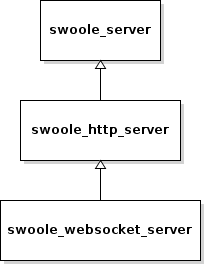
\includegraphics[scale=0.5]{swoole_server.png}
\caption{swoole\_server的继承关系}
\end{figure}

\begin{compactitem}
\item swoole\_http\_server是swoole\_server的子类,内置了Http的支持;
\item swoole\_websocket\_server是swoole\_http\_server的子类,在Http基础上内置了WebSocket的支持。
\end{compactitem}

Swoole的网络IO部分基于epoll/kqueue事件循环,因此全异步非阻塞执行,而且业务逻辑部分使用多进程同步阻塞方式来运行,从而既保证了Server能够应对高并发和大量TCP连接,又能够保证业务代码仍然可以简单地编写。





\subsection{swoole\_http\_server}




\begin{lstlisting}[language=bash]

\end{lstlisting}


\begin{lstlisting}[language=bash]

\end{lstlisting}

\begin{lstlisting}[language=bash]

\end{lstlisting}

\subsection{swoole\_websocket\_server}


\begin{lstlisting}[language=bash]

\end{lstlisting}




\begin{lstlisting}[language=bash]

\end{lstlisting}


\section{swiftmailer}


PHP直接使用SMTP协议来同步发送邮件的速度太慢,所以需要基于Swoole等来实现邮件的异步发送。



大概来说,Swoole服务器端程序以cli模式并运行在守护进程模式,然后再通过一个客户端去连接服务器端并通知发送邮件,服务器端在收到信息后过回调函数,执行相应的程序来实现邮件的异步发送。

\subsection{MailServer}

使用composer安装SwiftMailer。

\begin{lstlisting}[language=bash]
$ composer require swiftmailer/swiftmailer
\end{lstlisting}

使用Swoole服务器程序来响应客户端的请求并通过swiftmailer发送邮件。


\begin{lstlisting}[language=bash,basicstyle=\ttfamily\footnotesize]
<?php
/**
 * @author 
 * @created 2015/10/18 18:20
 */
require __DIR__ . '/vendor/autoload.php';

class MailServer
{
	const MAIL_USERNAME = 'no-reply@bz-inc.com';
	const MAIL_PASSWORD = 'p@$$w';
	
	private $logger = null;
	private $server = null;
	
	public function __construct()
	{
		$this->server = new swoole_server('0.0.0.0',9501);
		$this->server->set(
			[
				'worker_num'=>8,
				'daemonize'=>false,
				'max_request'=>100000,
				'dispatch_mode'=>2,
				'debug_mode'=>1
			]
		);
		
		$this->server->on('Start',[$this,'onStart']);
		$this->server->on('Connect',[$this,'onConnnect']);
		$this->server->on('Receive',[$this,'onReceive']);
		$this->server->on('Close',[$this,'onClose');
		
		$this->server->start();
	}
	
	public function onStart()
	{
		//
	}
	
	public function onConnect($server,$descriptors,$fromId)
	{
		//
	}
	
	public function onReceive(swoole_server $server,$descriptors,$fromId,$data)
	{
		$msg=json_decode($data,true);
		$sent=$this->sendMail($msg['address'],$msg['subject'],$msg['body']);
		printf("%s mail is sent.\n",$sent);
	}
	
	public function onClose($server, $descriptors,$fromId)
	{
		//
	}
	
	public function sendMail($address,$subject,$body)
	{
		$body=htmlspecialchars_decode($body);
		$transport=Swift_SmtpTransport::newInstance('smtp.partner.outlook.cn',587,'tls');
		$transport->setUsername(self::MAIL_USERNAME);
		$transport->setPassword(self::MAIL_PASSWORD);
		$mailer=Swift_Mailer::newInstance($transport);
		
		$message=Swift_Message::newInstance();
		$message->setFrom([self::MAIL_USERNAME=>'班砖网络']);
		$message->setTo($address);
		$message->setSubject($subject);
		$message->addPart($body,'text/html');
		$message->setBody($body);
		
		return $mailer->send($message);
	}
}
$server=new MailServer();
\end{lstlisting}


在配置好PHP以及Swoole后,使用cli启动服务端:

\begin{lstlisting}[language=bash]
$ php mail_server.php
\end{lstlisting}

如果需要让服务端在后台执行,可以修改配置数组\texttt{'daemonize' => false}为\texttt{'daemonize' => true}。


\subsection{MailClient}

使用client连接server并发送数据。




\begin{lstlisting}[language=bash]
<?php
/**
 * @author
 * @created 2015/10/18 18:40
 */
class MailClient
{
	private $client;
	public function __construct(){
		$this->client=new swoole_client(SWOOLE_SOCK_TCP);
	}
	
	public function connect(){
		if(!$this->client->connect('0.0.0.0',9501,1)){
			throw new CException(sprintf('Swoole Error: %s',$this->client->errCode));
		}
	}
	
	public function send($data)
	{
		if($this->client->isConnect()){
			if(!is_string($data)){
				$data=json_encode($data);
			}
			return $this->client->send($data);
		}else{
			throw new CException('Swoole Server does not connected.');
		}
	}
	
	public function close(){
		$this->client->close();
	}
}
\end{lstlisting}


\subsection{MailInstance}


\begin{lstlisting}[language=bash]
$data=array(
	'address'=>$mails,
	'subject'=>$subject,
	'body'=>htmlspecialchars($body)
);

$mailClient=new MailClient();
$mailClient->connect();

if($mailClient->send($data)){
	echo 'success';
}else{
	echo 'fail';
}

$mailClient->close();
\end{lstlisting}





\begin{lstlisting}[language=bash]

\end{lstlisting}




\begin{lstlisting}[language=bash]

\end{lstlisting}



\chapter{Client}

swoole\_client是TCP/UDP客户端,支持同步并发调用,也支持异步事件驱动。


\begin{lstlisting}[language=bash]

\end{lstlisting}




\begin{lstlisting}[language=bash]

\end{lstlisting}




\begin{lstlisting}[language=bash]

\end{lstlisting}


\chapter{Event}

EventLoop API\footnote{eventloop接口仅可用于socket类型的文件描述符,不能用于磁盘文件读写。},让用户可以直接操作底层的事件循环,将socket,stream,管道等Linux文件加入到事件循环中。


\section{swoole\_event}



\begin{lstlisting}[language=bash]

\end{lstlisting}




\begin{lstlisting}[language=bash]

\end{lstlisting}




\begin{lstlisting}[language=bash]

\end{lstlisting}


\chapter{Async}




\section{swoole\_async}



\begin{lstlisting}[language=bash]

\end{lstlisting}




\begin{lstlisting}[language=bash]

\end{lstlisting}




\begin{lstlisting}[language=bash]

\end{lstlisting}


\chapter{Process}


共享内存的性能虽然很好,但是存在安全问题,需要读写时加锁。

\begin{compactitem}
\item 锁的粒度过大会导致只有一个线程在运行。
\item 锁太复杂又会有死锁问题。
\end{compactitem}



\section{swoole\_process}

进程管理模块,可以方便的创建子进程,进程间通信,进程管理。

与Node.js的网络库本身没有提供多进程/多线程的实现的情况不同,swoole用户不需要自己手动管理进程的创建与回收,swoole内核根据配置文件自动完成,Node.j开发者需要自行创建进程,或者通过cluster来利用多核,否则只能使用单线程。






\begin{lstlisting}[language=bash]

\end{lstlisting}




\begin{lstlisting}[language=bash]

\end{lstlisting}




\begin{lstlisting}[language=bash]

\end{lstlisting}

\chapter{Buffer}



\section{swoole\_buffer}

强大的内存区管理工具,像C一样进行指针计算,又无需关心内存的申请和释放,而且不用担心内存越界,底层全部做好了。

\begin{lstlisting}[language=bash]

\end{lstlisting}




\begin{lstlisting}[language=bash]

\end{lstlisting}






\chapter{Table}



\section{swoole\_table}


swoole\_table是基于共享内存和自旋锁实现的超高性能内存表\footnote{swoole\_table的性能可以达到单线程每秒读写50W次。},可以彻底解决线程,进程间数据共享,加锁同步等问题。




\begin{lstlisting}[language=bash]

\end{lstlisting}





\begin{lstlisting}[language=bash]

\end{lstlisting}





\begin{lstlisting}[language=bash]

\end{lstlisting}




\begin{lstlisting}[language=bash]

\end{lstlisting}




\begin{lstlisting}[language=bash]

\end{lstlisting}




\begin{lstlisting}[language=bash]

\end{lstlisting}




\begin{lstlisting}[language=bash]

\end{lstlisting}




\begin{lstlisting}[language=bash]

\end{lstlisting}




\begin{lstlisting}[language=bash]

\end{lstlisting}





\begin{lstlisting}[language=bash]

\end{lstlisting}




\begin{lstlisting}[language=bash]

\end{lstlisting}




\begin{lstlisting}[language=bash]

\end{lstlisting}




\begin{lstlisting}[language=bash]

\end{lstlisting}




\begin{lstlisting}[language=bash]

\end{lstlisting}




\begin{lstlisting}[language=bash]

\end{lstlisting}




\begin{lstlisting}[language=bash]

\end{lstlisting}




\begin{lstlisting}[language=bash]

\end{lstlisting}




\begin{lstlisting}[language=bash]

\end{lstlisting}




\begin{lstlisting}[language=bash]

\end{lstlisting}




\begin{lstlisting}[language=bash]

\end{lstlisting}




\begin{lstlisting}[language=bash]

\end{lstlisting}




\begin{lstlisting}[language=bash]

\end{lstlisting}




\begin{lstlisting}[language=bash]

\end{lstlisting}





\begin{lstlisting}[language=bash]

\end{lstlisting}




\begin{lstlisting}[language=bash]

\end{lstlisting}






\begin{lstlisting}[language=bash]

\end{lstlisting}




\begin{lstlisting}[language=bash]

\end{lstlisting}




\begin{lstlisting}[language=bash]

\end{lstlisting}




\begin{lstlisting}[language=bash]

\end{lstlisting}




\begin{lstlisting}[language=bash]

\end{lstlisting}




\begin{lstlisting}[language=bash]

\end{lstlisting}




\begin{lstlisting}[language=bash]

\end{lstlisting}




\begin{lstlisting}[language=bash]

\end{lstlisting}




\begin{lstlisting}[language=bash]

\end{lstlisting}




\begin{lstlisting}[language=bash]

\end{lstlisting}





\begin{lstlisting}[language=bash]

\end{lstlisting}




\begin{lstlisting}[language=bash]

\end{lstlisting}




\begin{lstlisting}[language=bash]

\end{lstlisting}




\begin{lstlisting}[language=bash]

\end{lstlisting}




\begin{lstlisting}[language=bash]

\end{lstlisting}




\begin{lstlisting}[language=bash]

\end{lstlisting}




\begin{lstlisting}[language=bash]

\end{lstlisting}




\begin{lstlisting}[language=bash]

\end{lstlisting}




\begin{lstlisting}[language=bash]

\end{lstlisting}




\begin{lstlisting}[language=bash]

\end{lstlisting}




\begin{lstlisting}[language=bash]

\end{lstlisting}




\begin{lstlisting}[language=bash]

\end{lstlisting}





\begin{lstlisting}[language=bash]

\end{lstlisting}




\begin{lstlisting}[language=bash]

\end{lstlisting}



\begin{lstlisting}[language=bash]

\end{lstlisting}




\begin{lstlisting}[language=bash]

\end{lstlisting}




\begin{lstlisting}[language=bash]

\end{lstlisting}




\begin{lstlisting}[language=bash]

\end{lstlisting}




\begin{lstlisting}[language=bash]

\end{lstlisting}




\begin{lstlisting}[language=bash]

\end{lstlisting}




\begin{lstlisting}[language=bash]

\end{lstlisting}




\begin{lstlisting}[language=bash]

\end{lstlisting}





\begin{lstlisting}[language=bash]

\end{lstlisting}




\begin{lstlisting}[language=bash]

\end{lstlisting}




\begin{lstlisting}[language=bash]

\end{lstlisting}




\begin{lstlisting}[language=bash]

\end{lstlisting}




\begin{lstlisting}[language=bash]

\end{lstlisting}




\begin{lstlisting}[language=bash]

\end{lstlisting}




\begin{lstlisting}[language=bash]

\end{lstlisting}




\begin{lstlisting}[language=bash]

\end{lstlisting}




\begin{lstlisting}[language=bash]

\end{lstlisting}




\begin{lstlisting}[language=bash]

\end{lstlisting}




\begin{lstlisting}[language=bash]

\end{lstlisting}




\begin{lstlisting}[language=bash]

\end{lstlisting}




\begin{lstlisting}[language=bash]

\end{lstlisting}




\begin{lstlisting}[language=bash]

\end{lstlisting}





\begin{lstlisting}[language=bash]

\end{lstlisting}




\begin{lstlisting}[language=bash]

\end{lstlisting}

